\input{C:/NoteSchema/Templates/HomeworkTemp_1.tex}
\begin{document}
\title{A Simple \LaTeX\ Document}
\author{John Doe}
\date{\today}
\maketitle

% write a math integral for x^2
\newcommand{\problem}[1]{\textbf{Problem #1}}
\begin{equation}
\int_{0}^{3} x^2 dx = 9
\end{equation}

% plot \int_{0}^{3} x^2 dx on a graph
% shade the area under the curve
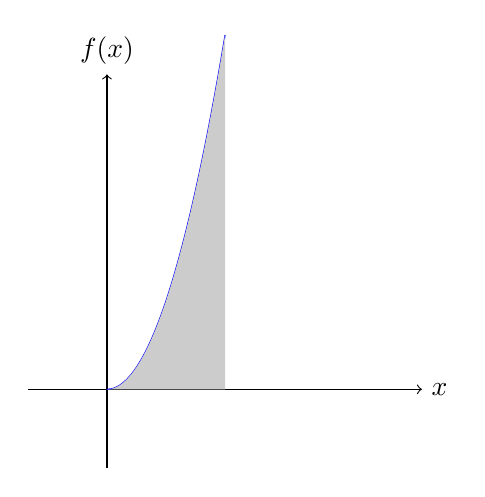
\begin{tikzpicture}
\draw[->] (-1,0) -- (4,0) node[right] {$x$};
\draw[->] (0,-1) -- (0,4) node[above] {$f(x)$};
\draw[scale=0.5,domain=0:3,smooth,variable=\x,blue] plot ({\x},{\x*\x});
\fill[gray!40!white,scale=0.5,domain=0:3,smooth,variable=\x] plot ({\x},{\x*\x}) -- (3,0) -- (0,0) -- cycle;
\end{tikzpicture}

\end{document}